% !TeX root = ../main.tex

\section{Caso di Studio}

\begin{frame}{Contesto Aziendale}
    \begin{figure}[H]
        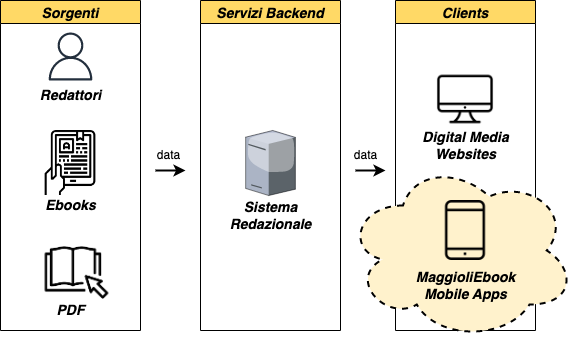
\includegraphics[width=0.7\textwidth]{img/contesto-aziendale.png}
    \end{figure}
    \begin{itemize}
        \item \textbf{Core Business}: Editoria e servizi per la pubblica amministrazione e professionisti
        \item \textbf{Necessità}: Sviluppare un nuovo metodo di accesso alle pubblicazioni digitali che sia più accessibile e pratico
        \item \textbf{Dominio}: Editoria digitale
    \end{itemize}
\end{frame}

\begin{frame}{Requisiti: Applicazione}
    \begin{columns}[onlytextwidth]
        \begin{column}{0.5\textwidth}
            \textbf{Tipologia}: E-Reader\\
            \vspace{5mm}
            \textbf{Funzionali}:
            \begin{itemize}
                \item Visualizzazione contenuti digitali
                \item Portabilità e leggibilità
                \item Ricerca pubblicazioni in base all'abbonamento dell'utente
                \item Personalizzazione tramite segnalibri e annotazioni
                \item Gestione preferiti
            \end{itemize}
            \vspace{5mm}
            \textbf{Tecnologici}:
            \begin{itemize}
                \item Versione Android e iOS
                \item Kotlin Multiplatform Mobile
            \end{itemize}
        \end{column}
        \begin{column}{0.45\textwidth}
             \begin{figure}[H]
                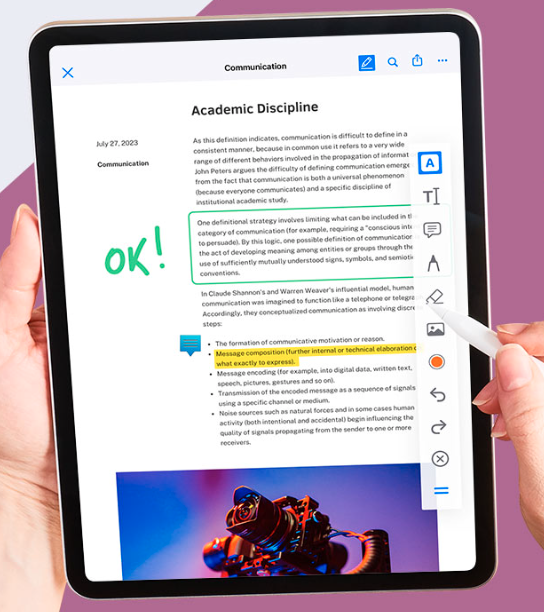
\includegraphics[width=1\textwidth]{img/e-reader.png}
            \end{figure}
        \end{column}
    \end{columns}
\end{frame}